% Style for a MSc paper at Warsaw School of Economics
% Michał Ramsza
% Friday, December 14, 2012

% --- document class and other global stuff ---------------------------
\documentclass[english, twoside, 12pt, a4paper]{article}



% --- packages --------------------------------------------------------
\usepackage{textcomp}
\usepackage{times}
\usepackage{amsmath}
\usepackage{amsfonts}
\usepackage{amssymb}
\usepackage{amsthm}
\usepackage[T1]{fontenc}
\usepackage[utf8]{inputenc}
\usepackage{graphicx}
\usepackage{xcolor}
\usepackage{enumitem}
\usepackage[english]{babel}
\usepackage[centering, left=3.5cm, right=2.5cm, textheight=24cm]{geometry}

% --- packages for citations ------------------------------------------
\usepackage{natbib}
\AtBeginDocument{\renewcommand{\harvardand}{and}}

% --- package for automatic insertion of R code -----------------------
\usepackage{listings}
\lstset{language=R,%
   numbers=left,%
   tabsize=3,%
   numberstyle=\footnotesize,%
   basicstyle=\ttfamily \footnotesize \color{black},%
   escapeinside={(*@}{@*)}}

% --- support for links -----------------------------------------------	
\usepackage{url}
\usepackage{hyperref}
\hypersetup{colorlinks=true,
            linkcolor=black,
            citecolor=darkgray,
            urlcolor=darkgray,
            pagecolor=darkgray}

% --- support for large tables and other stuff ------------------------	
\usepackage{longtable}
%\usepackage{subfigure} % this package will not work with subcaption package
\usepackage{float}
\usepackage{caption}
\usepackage{subcaption}
\usepackage{wrapfig}
\usepackage{pdflscape} % relevant for wide tables (rotating pages)

% --- support for game theory ------------------------------------------
\usepackage{sgame}

% --- support for no widows --------------------------------------------
\usepackage[defaultlines=4,all]{nowidow}

% --- definitions for environments -------------------------------------
\theoremstyle{definition}
    \newtheorem{condition}{Assumption}
    \newtheorem{example}{Example}      

\theoremstyle{plain}
    \newtheorem{definition}{Definition}    
    \newtheorem{proposition}{Proposition}
    \newtheorem{theorem}{Theorem}
    \newtheorem{cor}{Corollary}

\theoremstyle{remark}
    \newtheorem{remark}{Remark}

% --- other settings --------------------------------------------------
\linespread{1.5}
\frenchspacing
\sloppy
\allowdisplaybreaks[4]
\raggedbottom
\clubpenalty=10000
\widowpenalty=10000

% --- only if required ------------------------------------------------
\AtBeginDocument{\renewcommand*{\figurename}{Figure}}
\AtBeginDocument{\renewcommand*{\tablename}{Table}}

% --- changing definition of footnote ---------------------------------
\makeatletter
\renewcommand\footnotesize{%
   \@setfontsize\footnotesize\@ixpt{10}%
   \abovedisplayskip 8\p@ \@plus2\p@ \@minus4\p@
   \abovedisplayshortskip \z@ \@plus\p@
   \belowdisplayshortskip 4\p@ \@plus2\p@ \@minus2\p@
   \def\@listi{\leftmargin\leftmargini
               \topsep 4\p@ \@plus2\p@ \@minus2\p@
               \parsep 2\p@ \@plus\p@ \@minus\p@
               \itemsep \parsep}%
   \belowdisplayskip \abovedisplayskip
}
\makeatother


% ---------------------------------------------------------------------
\begin{document}

% --- strona tytulowa -------------------------------------------------
\begin{titlepage}
\centering


\includegraphics[width=0.66\textwidth]{logo.JPG}

\vspace*{0.5cm}
Studium licencjackie\\
\begin{flushleft}
Kierunek: Metody Ilościowe w Ekonomii i Systemy Informacyjne\\
%Specjalność: <specjalność> % w przypadku braku należy pominać
Forma studiów: Stacjonarne
\end{flushleft}

\vspace*{.5cm}
\rule{0cm}{1cm}\hfill
\begin{minipage}{9cm}
Imie i nazwisko autora: Kacper Mordarski\\
Nr albumu: 101247
\end{minipage}

\vspace*{1cm}
\begin{minipage}{12cm}
\centering
\Large
\textbf{<tytuł>}
\end{minipage}

\vspace*{2cm}
\rule{0cm}{1cm}\hfill
\begin{minipage}{9cm}
Praca licencjacka napisana\\
w Katedrze Matematyki i Ekonomii Matematycznej\\
pod kierunkiem naukowym\\
dr hab. Michała Ramszy
\end{minipage}

\vfill
Warszawa 2022
\end{titlepage}

\rule{1ex}{0ex}\clearpage

% --- table of contents -----------------------------------------------
\cleardoublepage
\tableofcontents

% --- chapter ---------------------------------------------------------
\cleardoublepage
\section{Introduction}
\subsection{General Introduction}

This paper aims to replicate, to an essential degree, the seminal paper on the emergence of cooperation, cf.~\cite{santos2005scale}. The secondary goal of this research is to provide the publicly available code allowing replication of the original results.

Tutaj jest drugi akapit. 

-----

either prove or disprove the research paper with title \mbox{\textbf{"Scale-Free Networks Provide a Unifying Framework for the Emergence of Cooperation"}}
 written by F.C. Santos and J. M. Pacheco and published in Physical Review Letters nr 95 (later on reffered to as "The Paper"). Regardless of the outcome this work is going to be useful
 because the above mentioned authors did not provide the code that was used to conduct the necessary simulations. Therefore goal is not only
 to disprove the above mantioned paper but also to provide readers with clear and easy to follow code. 
 
 \subsection{Description of The Paper}

The Paper was published in "Physical Review Letters" on 26th August 2005 and according to Google Scholar has been since cited over 1600 times. 
It clearly shows the magnitude of said paper and its groundbreaking character. This paper is presenting the results of simulations conducted by the authors and its 
implications for evolutionary game theory. The crucial thing to understand is that the authors of The Paper changed the approach to modelling such games by applying
Scale Free Networcs of Contacts (later on refferd to as "SF NOC's"). Its innovativeness lies in the never used before degree distribution of said graph. Before used
graphs had a degree distribution with a single peak. It means that every "player" could interact only with a fixed number of other "players". SF NOC's is said to 
perform better at modelling the actual, existing societies and networks. It complies with the rules of growth and preferential attachment (rich gets richer). If we 
analyse some actual networks - for example Twitter network, we observe that those with bigger count of "followers" are more likely to gain new ones than accounts 
with low count of "followers". One of the goals of The Paper was to compare results of simulations on different kinds of graphs. According to The Paper, players that 
occupy vertices of SF NOC are much more likely to cooperate than of any other graph. Those results came up both in Snowdrift game (later on reffered to as SG) and 
Prisoners Dilemma game (later on reffered to as PD). 


\subsection{A brief description of Snowdrift game and Prisoners Dilemma game}

\paragraph{Prisoners Dilemma Game}. The Prisoners Dillema game is a widely known problem in game theory and decision analysis. It shows that there exist situations in which the outcome is not optimal, even though players act in their own best interest. In the scope of our analysis, it is important to note that in the PD game, the best strategy is to defect, regardless of the opponent's choice. The game is parametrized as follows:
\begin{center}
\begin{game}{2}{2}
  & $C$    & $D$    \\
$C$ & $R,R$ & $S,T$  \\
$D$ & $T,S$ & $P,P$
\end{game}
\end{center}
where the values are given as follows:
\[
\begin{aligned}
T &= b > 1, \\
R &= 1, \\
P &= 0, \\
S &= 0, \\
1 &< b \le 2. 
\end{aligned}
\]
We see that the above restrictions order the parameters as follows:
\[
T > R > P = S
\]

\paragraph{Snowdrift Game.} The Snowdrift game represents a metaphore for cooperative interactions between players. Contrary to PD, the Snowdrift game stimulates the cooperative behaviour amongst
players. It doesn't make the deflection strategy totally inapplicable, but payoffs of this game favourizes cooperative behaviours more than the PD. The optimal strategy
is to cooperate when the other defects and to defect when the other cooperates.\\
\begin{center}
  \begin{game}{2}{2}
    & $C$    & $D$    \\
  $C$ & $R,R$ & $T,S$  \\
  $D$ & $S,T$ & $P,P$
  \end{game}
  \end{center}
  
  Where the parametrisation is as follows:\\
  \begin{center}
  \(T = \beta > 1 \)\\
  \(R = \beta - \frac{1}{2} \)\\
  \(S = 1 - \beta \)\\
  \(P = 0 \)
  

  \begin{center}
    \( T > R > P > S \)
  \end{center}


  \end{center}

\subsection{Simulations description}

Because of the nature of this paper (an attempt to clone the results of The Paper) our simulations must be conducted in a strickt accordance with the methods outlined
in The Paper. Therefore it is only natural that we must follow each step with the utmost care and diligence. According to The Paper we must conduct 100 simulations 
for each parametrisation. Each simulation is performed following those steps:\\
\begin{enumerate}
  \item Setting up the parameters which are needed to create SF NOC's (such as number of final vertices (population size), the avarage connectivity etc.).
  \item Choosing the parameters of game which is to be simulated (either PD or SG).
  \item Creating the randomly generated SF NOC (we use Barabasi - Albert model to do that). The SF NOC must be created in compliance with preferential attachment and 
  growth rules.
  \item Randomly distributing strategies amongst the population (SF NOC in this particular case). Each vertex can either get a cooperation or deflection strategy.
  \item Each pair of cooperator - deflector engages in a round of given game. In compliance with replicatory dynamics we keep track of cumulative payoffs for both 
  strategies so that "players" can adjust their strategies throughout the population. This step is repeated 11 000 times, each time is called "generation". The first 
  10 000 is so called "transient time".
  \item We collect results (equilibrium frequencies of cooperators and defectors) by avaraging over the last 1 000 generations.
\end{enumerate}

\subsection{Replicatory dynamics}

In our analysis we consider replicator to be a strategy in a game. The general idea is that replicators compete for dominance throughout the population. Payoffs of
their strategies represent their "fitness". It is important to note that each player can alter their strategy through inheritance. Attempt of inheritance occurs 
whenever on of the sites is updated. For the sake of an example lets say that the site that was just updated is a site x. The procedure is as follows:

\begin{enumerate}
  \item The site x is updated.
  \item A neighbour y is drawn at random among all k$_{x}$ neighbours
  \item if cumulative payoffs of y (P$_{y}$) is greater than cumulative payoffs of x (P$_{x}$), the chosen neighbour takes over site x with probability (P$_{i}$) given below.
\end{enumerate}


\begin{center}

\[
  P_{i} = \frac{(P_{y} - P_{x})}{Dk_{>}}
  \]
\end{center}
Where P$_{i}$ is the probability of the chosen neighour taking over the site x, P$_{y}$ is a cumulated payoffs of strategies y, P$_{x}$ is a cumulated payoffs 
of strategies x, k$_{>}$ is the largest between k$_{y}$ and k$_{x}$ (k$_{y}$ is a number of neighbours with a strategy y, k$_{x}$ is a number of neighbours with a 
strategy x), D depends on the game (it is equal to either T-S for PD or T-P for SG).\\


  % --- chapter ---------------------------------------------------------
\clearpage
\section{Basic things}

\subsection{Compiling \LaTeX files}

The \verb+.tex+ file is just a plain text file. It contains the \LaTeX formatting codes together with the content of a paper. To get a \verb+.pdf+ file you have to compile the \verb+.tex+ file using a sequence \verb+pdflatex+, \verb+biblatex+, \verb+pdflatex+, \verb+pdflatex+. This sequence is a default in most editors designed for use with \LaTeX.

\subsection{Basic formatting for a text}

Paragraphs are coded by an empty line. That is is you want to start a new paragraph it is enough to leave an empty line and start typing like that:
\begin{verbatim}
This is the first paragraph.

This is the next paragraph.
\end{verbatim}

Everything about the paragraph is formatted for you including all indents and spacings. Again, you don't have to take care of it manually.

Basic text formatting, e.g. bold face and italic, is achieved with the following commands: \verb+\textbf{}+, \verb+\textit{}+, \verb+\underline{}+, producing \textbf{text}, \textit{text}, \underline{text}. I suggest not overusing those commands!

Alignment is done through environments \verb+center+, \verb+flushleft+ and \verb+\flushright+ giving the following examples.

\begin{center}
  This is centered.
\end{center}

\begin{flushleft}
  This is aligned to the left.
\end{flushleft}

\begin{flushright}
  This is aligned to the right. 
\end{flushright}

In other environments it is possible to use \verb+\centering+ to center content of that environment (like in \verb+figure+ or \verb+table+ environments).

\subsection{Fonts and fonts' sizes}

You do not change fonts and fonts' sizes! Technically it can be done but I will reject this.

% --- chapter ---------------------------------------------------------
\clearpage
\section{Mathematics}

This is testing footnotes\footnote{This is a footnote. We can put some math here \( x^2 - f(x) = g(x^2) \) which is not encouraged but sometimes necessary. The other thing we can do is to put here an URL \url{https://tex.stackexchange.com/questions/249415/set-font-size-for-footnotes}. }.

\subsection{Basic mathematics}

There are two types of mathematics inside a \LaTeX{} document. The first one is the in-line mathematics and the displayed mathematics. The first one looks like this: \( F(x) = \int_{-\infty}^{x} f(\omega) d\omega \) with the code looking like this: \verb!\( F(x) = \int_{-\infty}^{x} f(\omega) d\omega \)!. The displayed mathematics looks like that
\[
F(x) = \int_{-\infty}^{x} f(\omega) d\omega
\]
with the code
\begin{verbatim}
\[
F(x) = \int_{-\infty}^{x} f(\omega) d\omega
\]
\end{verbatim}
As you can see the same code is formatted differently depending on the type of mathematics.

\subsection{Referencing mathematics and other things}

To reference mathematics (only displayed formulas) you use the \verb+equation+ environment with a \verb+\label{}+ within. The reference is done through the \verb+\ref{}+ command. The example is
\begin{equation}
\label{eq:this-is-very-important-equation}
F(x) = \int_{-\infty}^{x} f(\omega) d\omega.
\end{equation}
To reference the equation you use the \verb+\ref{}+ command giving (\ref{eq:this-is-very-important-equation}). The \verb+\label{}+ / \verb+\ref{}+ pair works for anything that can be referenced.

\subsection{Some more mathematical formulas}

Here are slightly more complex formulas. Let \( A  \) be a matrix
\[
A =
\left(
\begin{bmatrix}
1                   & \alpha^2       \\
2                   & \sqrt{\pi} - \log(x-\sin(y))
\end{bmatrix}^{2}
- 
\begin{bmatrix}
1                   & f(x)           \\
2                   & g(y)
\end{bmatrix}
\cdot
\begin{bmatrix}
x                                    \\
y
\end{bmatrix}
\right),
\]
where
\[
f(x) = 
\left\{
  \begin{aligned}
    \frac{1}{x}     & \quad \text{for \(x<-\frac{1}{2}\),} \\
    \frac{1}{1+x^2} & \quad \text{for \(x \geq -\frac{1}{2}\)}
  \end{aligned}
\right.
\]
and
\[
g(y) = \sin\left(\frac{\mathrm{\mathbf{E}}(X)}{\cos(y) + \log(y)}\right), 
\quad\text{where \( X \sim \mathrm{N}(0, \sigma)  \).}
\]

It is very easy to typeset a normal form game. Below is an example of such a game. 

\begin{game}{3}{3}
    & $L$    & $M$    & $H$    \\
$L$ & $16,9$ & $3,13$ & $0,3$  \\
$M$ & $21,1$ & $10,4$ & $-1,0$ \\
$H$ & $9,0$  & $5,-4$ & $-5,-15$
\end{game}

% --- chapter ---------------------------------------------------------
\clearpage
\section{Figures and tables}

Both figures and tables use the same ideas. To insert a table you use the \verb+table+ environment. This is an example of a simple table.

\begin{table}[hbt]
  \centering

  \captionsetup{margin=10pt,font=small,labelfont=bf,width=.8\textwidth}

  \caption[Short name for a table]{This is an example of a table.}
  \label{tab:exceptional-table}

\vspace*{2ex}

  \begin{tabular}{lccc}
    Name        & property 1 & property 2 & property 3 \\ \hline
    Michael     & 23         & 34         & --         \\
    John        & 34         & --         & 28         \\
    Mr. Niceguy & 123        & 231        & 312        \\ \hline
  \end{tabular}
\end{table}

Table~\ref{tab:exceptional-table} is a very simple table and much more is possible.

To insert a figure you need to have a figure. In the catalog there are two figures and the following is an example of the \verb+figure+ environment.

\begin{figure}[hbt]
  \centering

  \begin{subfigure}[t]{0.45\textwidth}
  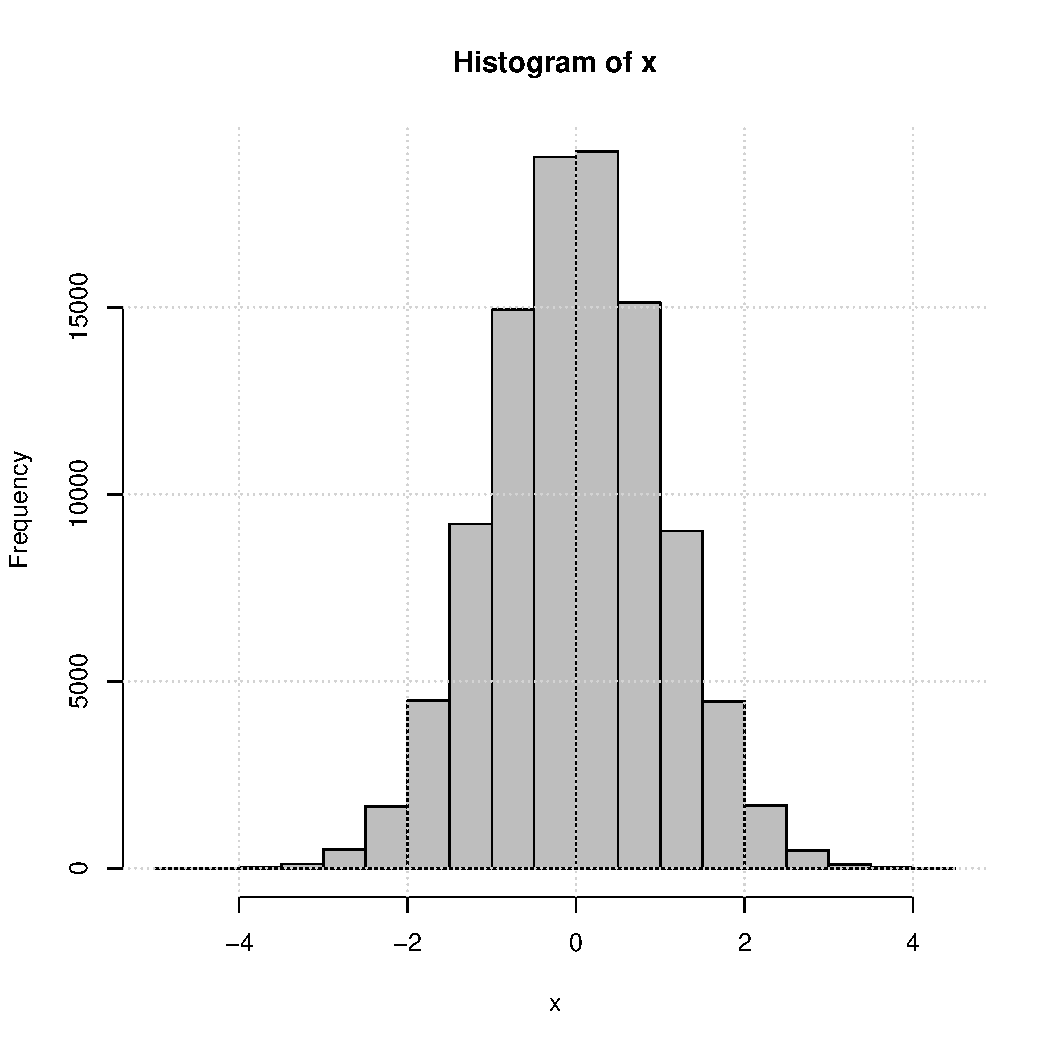
\includegraphics[width=\textwidth]{./figure-1}
  \end{subfigure}

  \captionsetup{margin=10pt,font=small,labelfont=bf,width=.8\textwidth}

  \caption[Short name]{This is just an example. \textit{Source:} own calculations.}\label{fig:xxx1}
\end{figure}

\begin{figure}[hbt]
  \centering
  \begin{subfigure}[t]{0.45\textwidth}
    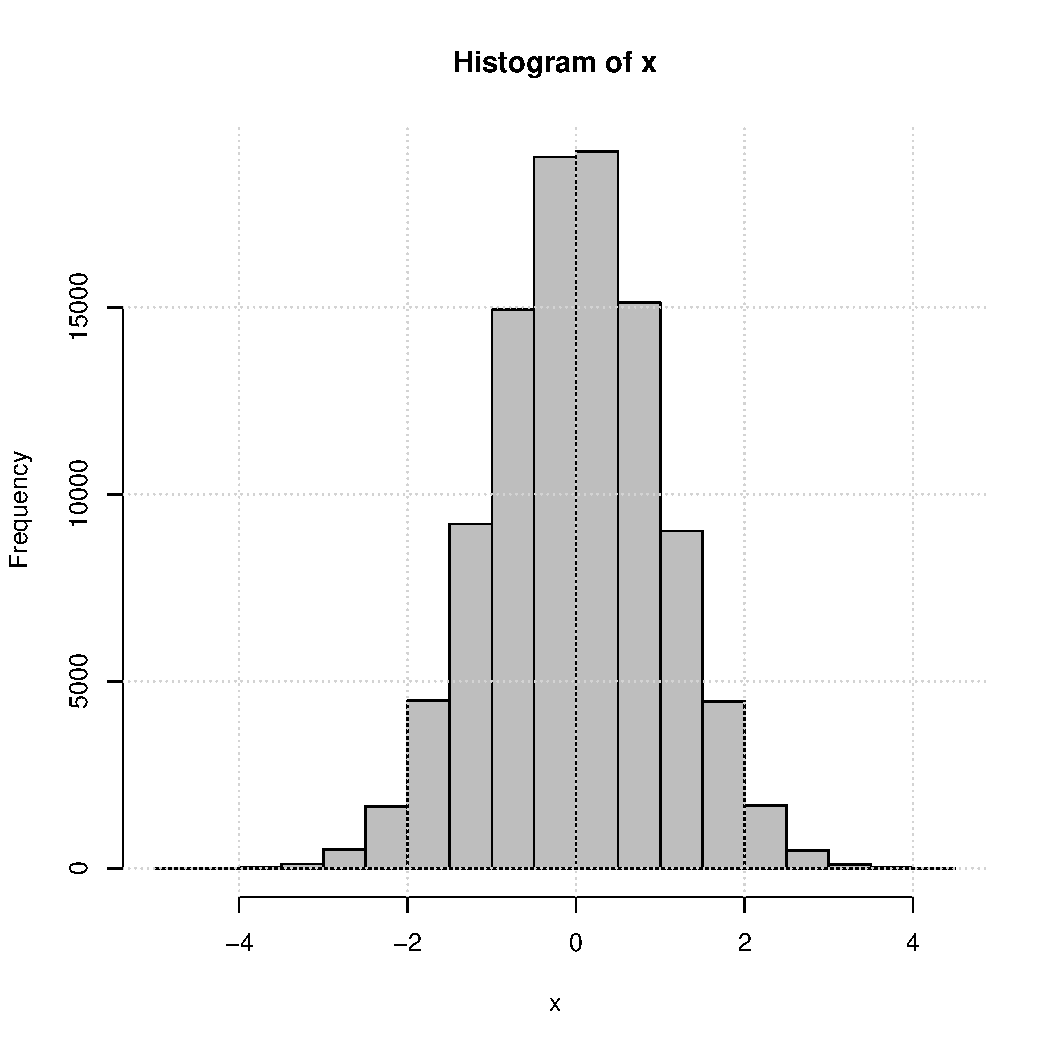
\includegraphics[width=\textwidth]{./figure-1}
    \caption{This is a caption for the first figure. This caption is wrapped at the right width and the hight is being compensated.}
    \label{fig:xxxa}
  \end{subfigure}
  \hfill
  \begin{subfigure}[t]{0.45\textwidth}
    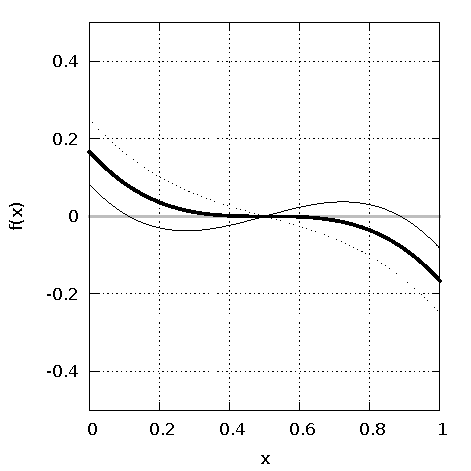
\includegraphics[width=\textwidth]{figure-2}
    \caption{This is another caption.}
    \label{fig:xxxb}
  \end{subfigure}
  
  \captionsetup{margin=10pt,font=small,labelfont=bf,width=.8\textwidth}

  \caption[Short caption 2]{This is the main caption and it is below the figures. \textit{Source:} own calculations}\label{fig:xxx}
\end{figure}

Figure~\ref{fig:xxx} is a slightly more complex than just a simple figure but it is useful to have such template. It is possible to refrence subfigures as \ref{fig:xxxa} and \ref{fig:xxxb}.

% --- chapter ---------------------------------------------------------
\clearpage
\section{Bibliography}

\begin{wrapfigure}{r}{.5\textwidth}
\centering

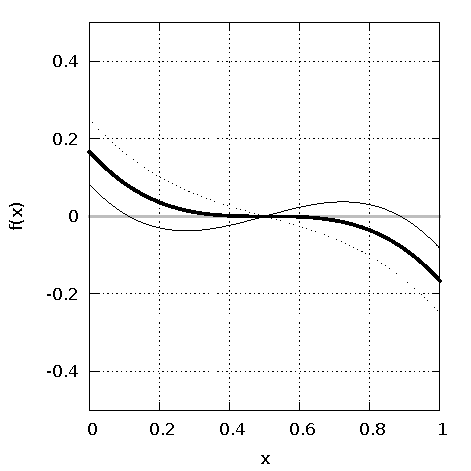
\includegraphics[width=.4\textwidth]{figure-2}

\captionsetup{margin=10pt,font=small,labelfont=bf,width=.42\textwidth}

  \caption[Short caption 2]{This is how one can wrap a text around a figure. \textit{Source:} own calculations}\label{fig:yyy}


\end{wrapfigure}

The content for the bibliography is in a different file named \verb+refs.bib+. You can change the name but then you have to change the information in this file from \verb+\bibliography{refs}+ to \verb+\bibliography{new-name}+ where \verb+new-name+ is the name of your file. The file \verb+refs.bib+ contains some examples for books and papers.

The process of citation is simple. The command  \verb+\cite{garland2010}+ gives this \cite{garland2010} and puts all information into the bibliography section  at the end. Everything is sorted and formatted for you so that you don't have to worry about this. An example of a paper with many authors is \cite{benaim2003} or \cite{osborne1998}. 

\begin{longtable}{rrrrr}
\caption{Binary variables used in the VAR model}\label{tab:1}     \\
  \hline
 t   & year & elections & crises & tax cuts                       \\ 
  \hline
  \endfirsthead
  \multicolumn{5}{c}%
{\tablename\ \thetable\ -- \textit{Continued from previous page}} \\
\hline
t    & year & elections & crises & tax cuts                       \\ 
\hline
\endhead
\hline \multicolumn{5}{r}{\textit{Continued on next page}}        \\
\endfoot
\hline
\endlastfoot
  1  & 1961 & 0         & 0      & 0                              \\ 
  2  & 1962 & 0         & 0      & 0                              \\ 
  3  & 1963 & 0         & 0      & 0                              \\ 
  4  & 1964 & 1         & 0      & 0                              \\ 
  5  & 1965 & 0         & 0      & 1                              \\ 
  6  & 1966 & 0         & 0      & 0                              \\ 
  7  & 1967 & 0         & 0      & 0                              \\ 
  8  & 1968 & 1         & 0      & 0                              \\ 
  9  & 1969 & 0         & 0      & 0                              \\ 
  10 & 1970 & 0         & 0      & 0                              \\ 
  11 & 1971 & 0         & 0      & 0                              \\ 
  12 & 1972 & 1         & 0      & 0                              \\ 
  13 & 1973 & 0         & 0      & 0                              \\ 
  14 & 1974 & 0         & 1      & 0                              \\ 
  15 & 1975 & 0         & 1      & 0                              \\ 
  16 & 1976 & 1         & 0      & 0                              \\ 
  17 & 1977 & 0         & 0      & 0                              \\ 
  18 & 1978 & 0         & 0      & 0                              \\ 
  19 & 1979 & 0         & 0      & 0                              \\ 
  20 & 1980 & 1         & 0      & 0                              \\ 
  21 & 1981 & 0         & 0      & 0                              \\ 
  22 & 1982 & 0         & 1      & 1                              \\ 
  23 & 1983 & 0         & 0      & 0                              \\ 
  24 & 1984 & 1         & 0      & 0                              \\ 
  25 & 1985 & 0         & 0      & 0                              \\ 
  26 & 1986 & 0         & 0      & 1                              \\ 
  27 & 1987 & 0         & 0      & 0                              \\ 
  28 & 1988 & 1         & 0      & 0                              \\ 
  29 & 1989 & 0         & 0      & 0                              \\ 
  30 & 1990 & 0         & 0      & 0                              \\ 
  31 & 1991 & 0         & 1      & 0                              \\ 
  32 & 1992 & 1         & 0      & 0                              \\ 
  33 & 1993 & 0         & 0      & 0                              \\ 
  34 & 1994 & 0         & 0      & 0                              \\ 
  35 & 1995 & 0         & 0      & 0                              \\ 
  36 & 1996 & 1         & 0      & 0                              \\ 
  37 & 1997 & 0         & 0      & 0                              \\ 
  38 & 1998 & 0         & 0      & 0                              \\ 
  39 & 1999 & 0         & 0      & 0                              \\ 
  40 & 2000 & 1         & 0      & 0                              \\ 
  41 & 2001 & 0         & 1      & 1                              \\ 
  42 & 2002 & 0         & 0      & 1                              \\ 
  43 & 2003 & 0         & 0      & 1                              \\ 
  44 & 2004 & 1         & 0      & 0                              \\ 
  45 & 2005 & 0         & 0      & 0                              \\ 
  46 & 2006 & 0         & 0      & 0                              \\ 
  47 & 2007 & 0         & 0      & 0                              \\ 
  48 & 2008 & 1         & 1      & 0                              \\ 
  49 & 2009 & 0         & 1      & 1                              \\ 
  50 & 2010 & 0         & 0      & 1                              \\ 
  51 & 2011 & 0         & 0      & 0                              \\ 
  52 & 2012 & 1         & 0      & 0                              \\ 
  53 & 2013 & 0         & 0      & 0                              \\ 
  54 & 2014 & 0         & 0      & 0                              \\ 
  55 & 2015 & 0         & 0      & 0                              \\ 
   \hline
\end{longtable}




% --- appendices ------------------------------------------------------
\appendix

% ---------------------------------------------------------------------
\clearpage
\section{Appendix: Some important stuff}

This appendix contains all the necessary important stuff, blah, blah, blah ...

\begin{landscape}
{\footnotesize
\begin{longtable}{lll}
\caption{Tutaj jest tytuł tablicy}\label{tab:nowatablica1}\\
\hline
Nazwa atrybutu & Wartości & Opis \\ 
\hline
\endfirsthead
\multicolumn{3}{c}%
{\tablename\ \thetable\ -- \textit{kontynuacja z poprzedniej strony}} \\
\hline
Nazwa atrybutu & Wartości & Opis \\
\hline
\endhead
\hline \multicolumn{3}{r}{\textit{kontynuowane na następnej stronie}} \\
\endfoot
\hline
\endlastfoot
chk\_acct & - & stan środków na rachunku bieżącym (jakościowa)\\ 
 & A11 & ... \textless 0 Marek Niemieckich\\  
 & A12 & 0 \textless ... \textless 200 Marek Niemieckich\\  
 & A13 & ... \textgreater 200 Marek Niemieckich\\  
 & A14 & brak rachunku bieżącego\\  
duration & - & czas trwania kredytu w miesiącach (numeryczna)\\  
history & - & przeszłość kredytowa (jakościowa)\\  
 & A30 & brak kredytów w historii/wszystkie kredyty poprawnie spłacone\\  
 & A31 & wszystkie kredyty poprawnie spłacone (zaciągnięte w tym banku)\\  
 & A32 & kredyty poprawnie spłacane po dzień dzisiejszy\\  
 & A33 & opóźnienia w poprzednich spłatach kredytu\\  
 & A34 & konto krytyczne/zaciągnięte kredyty w innych bankach\\  
purpose & - & cel (jakościowa)\\  
 & A40 & nowy samochód\\  
 & A41 & używany samochód\\  
 & A42 & meble\\  
 & A43 & telewizor\\  
 & A44 & urządzenia gospodarstwa domowego\\  
 & A45 & remont\\  
 & A46 & edukacja\\  
 & A47 & wakacje\\  
 & A48 & przekwalifikowanie\\  
 & A49 & biznes\\  
 & A410 & inne\\  
amount & - & kwota kredytu (numeryczna)\\  
say\_acct & - & saldo na rachunku oszczędnościowym/wartość posiadanych obligacji (jakościowa)\\  
 & A61 & ... \textless100 Marek Niemieckich\\  
 & A62 & 100 \textless= ... \textless 500 Marek Niemieckich\\  
 & A63 & 500 \textless= ... \textless 1000 Marek Niemieckich\\  
 & A64 & ... \textgreater= 1000 Marek Niemieckich\\  
 & A65 & nieznane/ brak oszczędności\\  
employment & - & czas zatrudnienia w obecnej pracy (jakościowa)\\  
 & A71 & brak zatrudnienia\\  
 & A72 & ... \textless 1 rok\\  
 & A73 & 1 \textless= ... \textless 4 lata\\  
 & A74 & 4 \textless= ... \textless 7 lat\\  
 & A75 & ... \textgreater= 7 lat\\  
install\_rate & - & wielkość raty jako procent rozporządzalnego przychodu (liczbowa)\\  
pstatus & - & płeć i stan cywilny (jakościowa)\\  
 & A91 & mężczyzna; rozwodnik/w separacji\\  
 & A92 & kobieta; rozwiedziona/ w separacji/ mężatka\\  
 & A93 & mężczyzna ; wolny\\  
 & A94 & mężczyzna ; żonaty/ wdowiec\\  
 & A95 & kobieta ; wolna\\  
other\_debtor & - & inni dłużnicy/ poręczyciele (jakościowa)\\  
 & A101 & brak\\  
 & A102 & współkredytobiorca\\  
 & A103 & poręczyciel\\  
property & - & własność/ mienie (jakościowa)\\  
 & A121 & nieruchomość\\  
 & A122 & (jeśli nie A121) umowa oszczędnościowa/ ubezpieczenie na życie\\  
 & A123 & (jeśli nie A121/A122) samochód lub inne\\  
 & A124 & nieznane\\  
timer\_resid & - & czas zamieszkania w aktualnym miejscu zamieszkania (liczbowa)\\  
age & - & wiek w latach (liczbowa)\\  
other\_install & - & inne zobowiązania ratalne (jakościowa)\\  
 & A141 & bank\\  
 & A142 & sklepy\\  
 & A143 & brak\\  
housing & - & warunki mieszkaniowe (jakościowa)\\  
 & A151 & wynajem\\  
 & A152 & własność\\  
 & A153 & zamieszkanie bez ponoszenia kosztów\\  
other\_credits & - & liczba aktualnych kredytów w tym banku (liczbowa)\\  
job & - & praca (jakościowa)\\  
 & A171 & bezrobotny/niewykwalifikowany; cudzoziemiec\\  
 & A172 & niewykwalifikowany; rezydent\\  
 & A173 & wykwalifikowany pracownik/urzędnik\\  
 & A174 & menadżer/ samozatrudniony/ wysocewykwalifikowany/ wyższy urzędnik\\  
num\_depend & - & liczba osób na utrzymaniu (liczbowa)\\  
telephone & - & telefon (jakościowa)\\  
 & A191 & brak\\  
 & A192 & tak, zarejestrowany pod nazwiskiem klienta\\  
foreign & - & pracownik zagraniczny (jakościowa)\\  
 & A201 & tak\\  
 & A202 & nie\\  
response & - & decyzja kredytowa\\  
 & 1 & tak\\  
 & 2 & nie\\ 
 \hline
\end{longtable}}
\end{landscape}



% --- bibliography ----------------------------------------------------
\clearpage
\bibliographystyle{agsm}
\bibliography{refs}

% --- abstract --------------------------------------------------------
\clearpage
\addcontentsline{toc}{section}{List of tables}
\listoftables

% --- abstract --------------------------------------------------------
\clearpage
\addcontentsline{toc}{section}{List of figures}
\listoffigures



% --- abstract --------------------------------------------------------
\clearpage
\addcontentsline{toc}{section}{Streszczenie}
\section*{Streszczenie}

Tutaj zamieszczają Państwo streszczenie pracy. Streszczenie powinno być długości około pół strony.


\end{document}


%%% Local Variables:
%%% mode: latex
%%% TeX-master: t
%%% End:
